%!TEX root = ../main.tex

% \begingroup
% \newgeometry{left=2.5cm,right=2.5cm,top=2.5cm,bottom=2.5cm}
% \part{Methodical}

% \endgroup
% A room without books is like a body without a soul.

%%%%%%%%%%%%%%%%%%%%%%%%%%%%%%%
%%%%%%%%%%%%%%%%%%%%%%%%%%%%%%%
%%%%%%%%%%%%%%%%%%%%%%%%%%%%%%%
\chapter{Methodical Modeling}

% \begin{textblock*}{.7\textwidth}(70mm-\offset,25mm-\offset)
%         \begin{fquote}[Mae West]
%                 You only live once, but if you do it right, once is enough.
%         \end{fquote}
% \end{textblock*}

\begin{textblock*}{.7\textwidth}(70mm-\offset,25mm-\offset)
        \begin{fquote}[Albert Einstein]
            All models are wrong, but some are useful.
        \end{fquote}
\end{textblock*}

%%%%%%%%%%%%%%%%%%%%%%%%%%%%%%%
%%%%%%%%%%%%%%%%%%%%%%%%%%%%%%%
\section{Transformer Equipment Modeling}


Some literature and fundamentals about transformers, control, stability assessment, fast-switching modules, and analysis in Python. % \todo{Hier steht ein Beispielkommentar.}

% \begin{figure}[h]
%         \centering
%         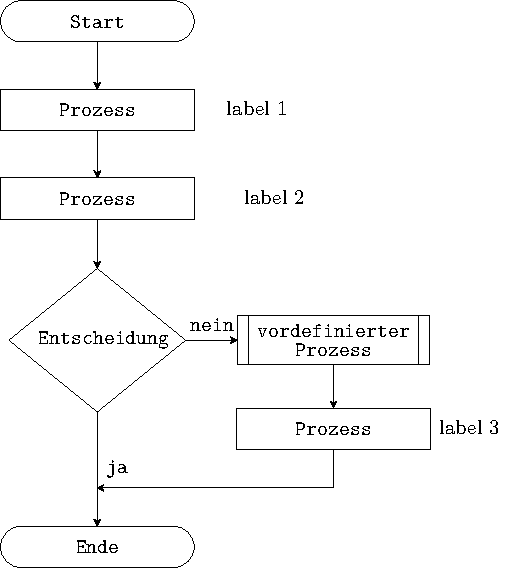
\includegraphics{tikz_graphics/images/programm.pdf}
%         \caption[Program plan proposal for determining the \acf{CCT}]{Program plan proposal for determining the \acf{CCT} $t_\mathrm{cc}$, critical power angle $\delta_\mathrm{cc}$ and the \acf{TDS} of the \acf{SMIB}-model; including the associated main function name}
%         \label{fig:program-plan}
% \end{figure}

\commenting{
        Things to mention:
        \begin{itemize}[nosep]
                \item First model: Admittance Matrix manipulations
                \item Second model: Current Injection Model
        \end{itemize}
}


%%%%%%%%%%%%%%%%%%%%%%%%%%%%%%%
\subsection{Implementing a $\Pi$-Representative Circuit with Variable Ratio}

% \commenting{Describe the current implementation of transformers in the Python framework.}
% \commenting{Follwing the description of the \glqq new\grqq implementation.}

\subsubsection{Mathematical Description and Definitions}

\commenting{
        Describe the Transformer circuit, the $\Pi$-model, simplification of impedances, relation to the specific side, ...
        \begin{enumerate}[nosep]
                \item Show the admittance matrix deduction process for placing the impedances on one side
                \item How to interprete $\underline{\vartheta}$; especially if complex and a mixture of longitudinal and angle ratio\\
                -> e.g. Asymmetrical shifter, vector groups, or only tapping on the current-voltage angle $\phi$
                \item Illustrate differences if the impedance relation is switching sides (Machowski vs. Kundur / Milano)\\
                -> refer the admittances to the lv or hv side: different definition of $\underline{\vartheta}$, different admittance matrix of the transformer
                \item Dependency of connections? (which side, step-up, step-down transformer?)
        \end{enumerate}
}

\subsubsection{Mathematical for MACHOWSKI / SIMULATION}

\commenting{
Similiar to the mentioned typical assumptions from \autocite{machowskiPowerSystemDynamics2020}
\begin{itemize}
        \item Neglecting (normally big) shunt branches in the circuit,
        \item Assuming the impedances on the HV and LV side are symmetrical (the same), and
        \item (\dots more?), 
\end{itemize}
these are considered in this paper as well. 

Procedure for accounting the Admittance Matrix:
\begin{enumerate}
        \item Set constraints as Ohms law for the admittance matrix and the tap ratio,
        \item Re-arrange equation to set currents and voltages independent of the transformer ratio, 
        \item calculate the series admittance and the shunt admittances after the given standard formula.
\end{enumerate}
\begin{align}
        \begin{bmatrix}
                \underline{I}_1 \\ \underline{I}_2
        \end{bmatrix}=
        \begin{bmatrix}
                \underline{Y}_{12} + \underline{Y}_{10} & -\underline{Y}_{12} \\ -\underline{Y}_{21} & \underline{Y}_{21} + \underline{Y}_{20}
        \end{bmatrix} \cdot
        \begin{bmatrix}
                \underline{U}_1 \\ \underline{U}_2
        \end{bmatrix}
\end{align}

\acs{OLTC} tap ratio definition:
\begin{align}
        \underline{\vartheta} &= 1 + k \cdot \Delta v \\[6pt]
        \text{with } k &\in [k_\mathrm{min};k_\mathrm{max}]; k_\mathrm{min} \equiv  -k_\mathrm{max}
\end{align}
Angle definition as multiplication to the tap ratio:
\begin{align}
        \underline{a}_\mathrm{T} &= \exp(j \cdot \phi \cdot \frac{\pi}{180})
\end{align}

}
\subsubsection{Mathematical for Paper ILYA and KUNDUR / MILANO}

\sidenote{Definition OLTC ratio}
\commenting{
        Relavant points for the definition of the OLTC ratio:
        \begin{itemize}[nosep]
                \item Complex vs. Rational number: Angle or Asymetric shifter
                \item How can angles and logitudinal ratios be mathematically expressed?
                \item How to understand when Relation to hv or lv side?
        \end{itemize}
}
The \acs{OLTC} ratio $\underline{\vartheta}$ when placing the replacement impedance $\underline{Z}_\mathrm{T}$, respectively the replacement admittance $\underline{Y}_\mathrm{T}$, on the high voltage side is defined as:
\begin{align}
        \underline{\vartheta} &= 1 + k \cdot \Delta v \label{eq:tap-ratio-hv} \\[6pt]
        \text{with } k &\in [k_\mathrm{min};k_\mathrm{max}]; k_\mathrm{min} \equiv  -k_\mathrm{max} \label{eq:tap-pos}
\end{align}
Within this definition, $k_\mathrm{min}$ defines the minimum tap position, $k_\mathrm{max}$ the maximum \acs{OLTC} postition. When relating the replacement impedance to the low voltage side, the tap ratio is defined differently, while looking at the tap position in \autoref{eq:tap-pos} in the same manner.
\begin{align}
        \underline{\vartheta} &= \frac{1}{1 + k \cdot \Delta v} \label{eq:tap-ratio-lv}
\end{align}

\sidenote{Representation of\\Vector Groups}
Voltage angle shifting through the influence of vector groups, meaning a different wiring and thus magnetic coupling of the transformer can be expressed within the transformer model. By mathematically applying a turning vector with the length of one to the overall tap ratio, this can be included in the model. Mathematical, this is expressed by the following equation. The characteristic number $n_\mathrm{T}$ is relating to to angle, with one step being equal to $30^\circ$ angle ratio.
\begin{align}
        \underline{a}_\mathrm{T} &= \exp(j \cdot n_\mathrm{T} \cdot \frac{\pi}{6}) \label{eq:vector-group}
\end{align}

\sidenote{Ideal vs. asymmetric ratio}
\commenting{Just briefly desribe the influence of an asymetric vs. an ideal transformer. Why the difference and how the representation could work.}
\begin{figure}[htb!]
        \centering
        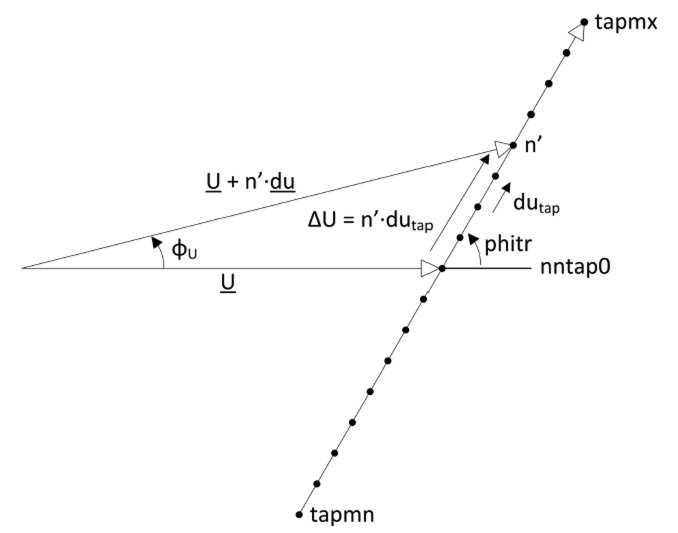
\includegraphics[width=.7\linewidth]{images/modeling/asymetric_ratio_vector.png}
        \caption[Illustration of the tap ratio vector for an ideal and an asymmetric transformer]{Illustration of the tap ratio vector for an ideal and an asymmetric transformer; from the \textcolor{ees_red}{\textbf{DIgSILENT Technical Reference Manual}} \dots \quelle}
        \label{fig:asymetric-ratio-vector}
\end{figure}

\subsubsection{Additional Algorithmics}

\commenting{
        \begin{itemize}[nosep]
                \item How to automatically determine switching direction?\\
                -> switchin direction dependent on what? (load-flow direction?)
                \item Controller set points: also dependent on load flow?
                \item How can I change the transformer control setpoints to be load flow dependent?
                \item How can I ensure, utilization of the transformer is not $>S_\mathrm{n}$?
        \end{itemize}
}

%%%%%%%%%%%%%%%%%%%%%%%%%%%%%%%
\subsection{Tap Changer Control Modeling}

\commenting{This is the description of the ideas, development, and implementation of a OLTC control scheme.}

\subsubsection{Discrete Control Loop}
\commenting{
        \begin{itemize}[nosep]
                \item Describe implementation
                \item Describe benefits / drawbacks
                \item Control scheme
                \item Switching logic and behavior (voltage tracking)
        \end{itemize}
}

\sidenote{General aspects and references}
This control method represents the currently most used and thus representative control scheme for \acsp{OLTC}. With the mechanic nature of the switching mechanism, the control look can only access discrete ratios within time frames of around a few seconds. Such a discrete control loop is described by \textcite{milanoHybridControlModel2011,milanoPowerSystemModelling2010}. A scheme of this control loop is shown in \autoref{fig:discrete-control-loop}.

\begin{figure}[htb!]
        \centering
        \missingfigure{Discrete control loop}
        \caption{Discrete control loop of an \acs{OLTC}; scheme based on \textcite{milanoHybridControlModel2011}}
        \label{fig:discrete-control-loop}
\end{figure}

This control loop type is beneficial due to its accurate representability of current \acs{OLTC} abilities. It gains access to assess stability within simulation environments, as analytical methods are not suited.

A negative aspect of a discrete control loop is the missing opportunity of generating a transfer function. This blocks the stability assessment with standard control engineering methods. Further, popular analysis methods like eigenvalue analysis is not possible, due to the lack of possibility to form derivatives.

% \lstinputlisting[caption={Output Function of the discrete OLTC controller},captionpos=b,style=style-python,label=lst:oltc-discrete]{images/code/oltc-discrete.py}

\sidenote{Implementation\\Structure}
\commenting{The structure of the implementation is illustrated in the block diagram of \autoref{fig:discrete-oltc-implementation}. The controller is actively chainging the algebraic funtions of the simulation environment, therefore it is quasi dynamic. The controller output logic is called, when updating the admittance matrix of the transformer. Additionally, the differential functions of the connected simple controllers, like integrators, PT1-blocks, etc., are called by the solver and are thus part of the differential equations. The logic determines the physical interpretation of the \acs{OLTC}, and therefore
\begin{enumerate}
        \item If the OLTC has to switch,
        \item When the switching operation is finished, and
        \item What the current, or in case after a switching the new, tap ratio is.
\end{enumerate}
It is important to note, that this structure relies on the calculation of the dynamic admittance matrix on each time step.}

\begin{figure}[htb!]
        \centering
        \missingfigure{Implementation structure of the discrete OLTC controller}
        \caption[Implementation structure of the discrete OLTC controller]{Implementation structure of the discrete OLTC controller}
        \label{fig:discrete-oltc-implementation}
\end{figure}

\sidenote{Output logic}
The output of the controller is based on the following logic.

\sidenote{Characterization plot and validation}

% \lstinputlisting[caption={Output Function of the discrete OLTC controller 2},captionpos=b,style=style-python,label=lst:oltc-discrete2]{images/code/oltc-discrete.py}

\subsubsection{Continous Control Loop}

\begin{figure}[htb!]
        \centering
        \includegraphics[width=.7\linewidth]{development_files/validation/data/oltc_control_characterization.pdf}
        \caption[Characterization of the OLTC control loops]{Characterization of the OLTC control loop; the input function simulates the to be regulated voltage, the output functions are characterized by $o(t)=i(t) \cdot \underline{\vartheta}_\mathrm{trafo}$}
        \label{fig:oltc-control-characterization}
\end{figure}

\subsubsection{Control Schemes for the Fast Switching module}
\commenting{
        \begin{itemize}[nosep]
                \item Describe implementation
                \item Describe benefits / drawbacks
                \item Control scheme
                \item Switching logic and behavior (voltage tracking)
        \end{itemize}
}
\sidenote{Functional basics of a \acs{FSM}}
Describe the operational logic and structure of the \acf{FSM} first.

\sidenote{Control logic}
A control logic for a so called \acs{FSM} has been presented from \textcite{burlakinEnhancedVoltageControl2024}, and illustrated in \autoref{fig:fsm-control-loop}.

\begin{figure}[htb!]
        \centering
        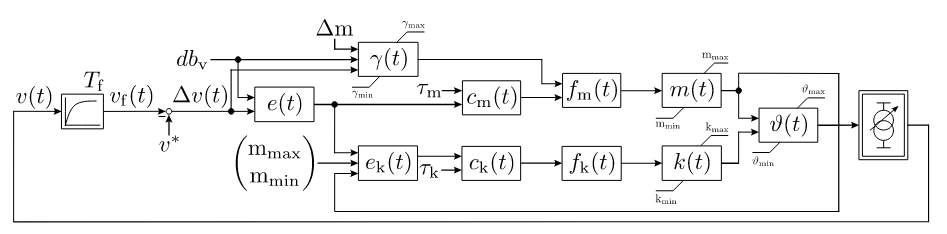
\includegraphics[width=\textwidth]{modeling/fsm_control_scheme.png}
        \caption[Control loop of a \acf{FSM}]{Control loop of a \acs{FSM}; scheme based on \textcite{burlakinEnhancedVoltageControl2024}}
        \label{fig:fsm-control-loop}
\end{figure}

\sidenote{Implementation\\differences}
However, the implementation logic in Python is slightly differing from the presented scheme in \autocite{burlakinEnhancedVoltageControl2024}, simply for not overcomplication of the code and therefeore debugging. The implementation is similar to the afore discussed one of a standard \acs{OLTC} controller. 

\sidenote{Characterization and validation}

\subsubsection{Discrete Control Loop as most Representative}
A continous control loop for a \acs{FSM} is presented within \textcite{burlakinEnhancedVoltageControl2024,burlakinEnhancingVariableShunt2024}. Similar to the solely \acs{OLTC} loop, it represents the real behavior best, but is obstructive for stability assessments. The scheme of the logic is shown in \autoref{fig:fsm-continuous-control-loop}.

\begin{figure}[htb!]
        \centering
        \missingfigure{Continuous control loop of a FSM}
        \caption{Continuous control loop of a \acs{FSM}; scheme based on \textcite{burlakinEnhancedVoltageControl2024}}
        \label{fig:fsm-continuous-control-loop}
\end{figure}

\subsubsection{Continuous Control Loop for best Stability Assessment}

%%%%%%%%%%%%%%%%%%%%%%%%%%%%%%%
\subsection{Experimental: Extended Ideas and Improvements}

\subsubsection{Operational Oriented FSM Control}

\subsubsection{Alternative Tap Skipping Logic}

\subsubsection{Varying the Voltage Setpoint and Target Calculation}

\commenting{Here, another idea of control target creation shall be mentioned. Instead of a fixed bus voltage reference, the difference of both bus voltages is considered. Further, the sign of that difference is used to determine the direction of the tap change.}

%%%%%%%%%%%%%%%%%%%%%%%%%%%%%%%
%%%%%%%%%%%%%%%%%%%%%%%%%%%%%%%
\section{Supplementary Modeling and Advancements}

As the python framework is currently missing some representations of components, this chapter aims to describe the implementation of those. Mainly focussing on source and load models, as the later considered test, benchmark, and use case networks require alternative behaviors. 

%%%%%%%%%%%%%%%%%%%%%%%%%%%%%%%
\subsection{ZIP Load Model}

\commenting{Why important?}

Mostly, a polynomial load model is used. It is called ZIP-model, as there are individual contributions to constant impedance $\underline{Z}$, constant current $\underline{I}$, and constant power $P$, or respectively $Q$, are considered. The model is described by \textcite{IEEEGuideLoad2022}. Either two ways of mathematical description are considered valid, dependent on the allowed influence of the frequency deviation. The use of periodized phasor representation, typical for a \acs{RMS} simulation, is missing or often neglecting this frequency information. Therefore the set of \autoref{eq:zip-1} and \autoref{eq:zip-2} is considered sufficient and implemented in the Python framework.
\begin{align}
        P&=P_n \cdot \Bigg[ p_1 \Bigg(\frac{U}{U_n}\Bigg)^2 + p_2 \Bigg(\frac{U}{U_n}\Bigg) + p_3 \Bigg] \label{eq:zip-1} \\[12pt]
        Q&=Q_n \cdot \Bigg[ q_1 \Bigg(\frac{U}{U_n}\Bigg)^2 + q_2 \Bigg(\frac{U}{U_n}\Bigg) + q_3 \Bigg] \label{eq:zip-2} \\[12pt]
        \text{with} \quad &p_i \in [0,1] \quad \text{and} \quad q_i \in [0,1] \notag
\end{align}

\commenting{Characteristics?}

\begin{figure}[htb!]
        \centering
        \includegraphics[width=\linewidth]{development_files/data/zip-load_characterization_full.pdf}
        \caption[Characterization of the ZIP load model]{Characterization of the ZIP load model; with (upper) the result of the impedances dependent on the voltage at the connected bus, and (lower) the resulting power consumption of the different models, representative only the real power $P$}
        \label{fig:zip-charac}
\end{figure}

\commenting{How does it look like in the simulation environment?}

\begin{align}
        P&=P_n \cdot \Bigg[ p_1 \Bigg(\frac{U}{U_n}\Bigg)^2 + p_2 \Bigg(\frac{U}{U_n}\Bigg) + p_3 \Bigg] \cdot (1+k_{pf} \Delta f) \label{eq:zip-with-f-1} \\[12pt]
        Q&=Q_n \cdot \Bigg[ q_1 \Bigg(\frac{U}{U_n}\Bigg)^2 + q_2 \Bigg(\frac{U}{U_n}\Bigg) + q_3 \Bigg] \cdot (1+k_{qf} \Delta f) \label{eq:zip-with-f-2} \\[12pt]
        \text{with} \quad &\sum_{i=1}^{3} p_i =1 \quad \text{and} \quad \sum_{i=1}^{3} q_i =1 \notag
\end{align}

Although the subset of \autoref{eq:zip-with-f-1} and \autoref{eq:zip-with-f-2} would consider a relation to the frequency at the given time, it is not used. The use of periodized phasor representation, typical for a \acs{RMS} simulation, is missing this information in the framework diffpssi. Therefore the set of \autoref{eq:zip-1} and \autoref{eq:zip-2} is implemented in the Python framework. It has to be mentioned, because the comparison tool PowerFactory is using this load model, though in some parts of the simulation results are showing a slightly bigger error.

%%%%%%%%%%%%%%%%%%%%%%%%%%%%%%%
\subsection{Induction Machine Models}

As one of the most important loads to consider, especially for many load driven instability mechanisms, the \ac{IM} is a crucial component, \quelle

\commenting{
        Just briefly:
        \begin{itemize}[nosep]
                \item Why is it crucial?
                \item How do the instability mechanisms work and look like?
                \item What are the different types of \acsp{IM} modeling (complete and dynamic, static, \dots)
        \end{itemize}
}

Three main ways of \acs{IM} modeling are relevant to mention in this section:
\begin{enumerate}
        \item Static model as introduced in \textcite{IEEEGuideLoad2022},
        \item a dynamic 'fixed-speed' \acs{IM} model, and
        \item a doubly fed \acs{IM} model.
\end{enumerate} 
The last ones are mentioned and further described in \textcite{machowskiPowerSystemDynamics2020}. Least model requires very detailed information, and shall be suitable for \acs{SMIB} models for machine behavior studies or similar. The second model is suitable for network analysis and machine behaviors. The first model applies for high perception of \acsp{IM} in total loading of the network. As referencing to \textcite{IEEEGuideLoad2022}, is is similar implemented as the before mentioned ZIP load model, considering characteristic equations for its real power $P$ and reactive power $Q$. Both models shall be described in the following section.

\subsubsection{Static Model of Induction Machines}

For this operational unit type is a detailed dynamic modeling possible. With some considerations, it can be sufficient, modeling this equipment just with the  The model is described by \textcite{IEEEGuideLoad2022} as formulated in following set of equations. %\autoref{eq:im-model}.

\begin{align}
        P&=\Bigg( R_\mathrm{s} + \frac{R_\mathrm{r}}{s} \Bigg) \cdot \frac{U^2}{\Big( R_\mathrm{s} + \frac{R_\mathrm{r}}{S} \Big)^2 + (X_\mathrm{\gamma s} + X_\mathrm{\gamma r})^2} \\[12pt]
        Q&=(X_\mathrm{\gamma s} + X_\mathrm{\gamma r}) \cdot \frac{U^2}{\Big( R_\mathrm{s} + \frac{R_\mathrm{r}}{S} \Big)^2 + (X_\mathrm{\gamma s} + X_\mathrm{\gamma r})^2} + \frac{U^2}{X_\mathrm{s}}
\end{align}
\mycomment[MK]{Is here really a difference between the two s in the equations?}

\commenting{Briefly describe the implementation.}

\subsubsection{Dynamic 'fixed-speed' Induction Machine model'}

\ai{\textbf{From ChatGPT:}

The dynamic model of \acsp{IM} is essential for accurately representing their behavior under various operating conditions. This model includes the differential equations that describe the machine's electrical and mechanical dynamics. The equations are typically derived from the machine's equivalent circuit and can be expressed in the d-q reference frame.

The dynamic model can be represented by the following set of equations:

\begin{align}
        \frac{\dd\psi_\mathrm{d}}{dt} &= v_\mathrm{d} - R_\mathrm{s} i_\mathrm{d} + \omega \psi_\mathrm{q} \\[12pt]
        \frac{\dd\psi_\mathrm{q}}{dt} &= v_\mathrm{q} - R_\mathrm{s} i_\mathrm{q} - \omega \psi_\mathrm{d} \\[12pt]
        \frac{\dd\omega}{dt} &= \frac{1}{J} (T_m - T_e - B \omega)
\end{align}

where:
\begin{itemize}
        \item $\psi_\mathrm{d}, \psi_\mathrm{q}$ are the d-q axis flux linkages
        \item $v_\mathrm{d}, v_\mathrm{q}$ are the d-q axis voltages
        \item $i_\mathrm{d}, i_\mathrm{q}$ are the d-q axis currents
        \item $R_\mathrm{s}$ is the stator resistance
        \item $\omega$ is the rotor angular velocity
        \item $T_\mathrm{m}$ is the mechanical torque
        \item $T_\mathrm{e}$ is the electromagnetic torque
        \item $J$ is the moment of inertia
        \item $B$ is the damping coefficient
\end{itemize}

The electromagnetic torque $T_e$ can be calculated as:

\begin{align}
        T_e = \frac{3}{2} p (\psi_d i_q - \psi_q i_d)
\end{align}

where $p$ is the number of pole pairs.

This dynamic model allows for the simulation of the \acsp{IM} transient response to changes in voltage, frequency, and load conditions. It is particularly useful for studying stability and control strategies in power systems.

}

\commenting{Briefly describe the implementation.}

% \subsection{PQ Source without Machine Dynamics}

% \todo[inline]{Necessary? Because one can use just an inverter at defined operation points}

% \commenting{Isn't that quite the same as the ZIP load model, but with inversed Power characteristics? Or is there more, for example when looking at a short circuit event\dots}

% \commenting{
%         These sections (per module / model) should contain roughly follwing information and / or structure:
%         \begin{enumerate}
%                 \item Why is this model important?
%                 \item How is it implemented?
%                 \item What are the characteristics (show in plots, description, etc.)?
%                 \item How does it look like in the simulation environment? -> Smaller example networks, like the \acs{SMIB} model; most likely combined with verification data of PowerFactory.
%         \end{enumerate}
% }


%%%%%%%%%%%%%%%%%%%%%%%%%%%%%%%
%%%%%%%%%%%%%%%%%%%%%%%%%%%%%%%
\section{Application of Voltage Stability}

%%%%%%%%%%%%%%%%%%%%%%%%%%%%%%%
\subsection{Influences of other device characteristics}

\commenting{
        Just look on other mutual influences in the power system (simulation), such as:
        \begin{itemize}[nosep]
                \item Load characteristics and types of modeling
                \item Maximum thermal currents of cables and operating components
                \item Asynchronous machines (or called \glqq induction motors\grqq?)
        \end{itemize}
}

%%%%%%%%%%%%%%%%%%%%%%%%%%%%%%%
\subsection{Observing the current state of the system}

\subsubsection{Static and Dynamic Indices}

\commenting{
        \begin{itemize}[nosep]
                \item Which indices can be implemented?
                \item Which make sense?
                \item Implementation and calculation of them?
        \end{itemize}
}

\subsubsection{Stability Monitoring}

\commenting{
        \begin{itemize}[nosep]
                \item Index combination and \glqq traffic light\grqq\~monitoring
                \item Restauration options and opportunities
                \item Local mapping
                \item Weak point identification
        \end{itemize}
}

% %%%%%%%%%%%%%%%%%%%%%%%%%%%%%%%
% \subsection{Wide-area control mechanisms}

% \commenting{
%         \begin{itemize}
%                 \item What influences could an interconnected information system have on curretn \glqq dumb transformer control\grqq?
%                 \item Reference voltages usually come from load flow analysis out of the back office (day-ahead); How can this be changed? How can transformers get more \glqq smart\grqq?
%         \end{itemize}
% }